\documentclass{apcalc}
\title{Unit 5: Analytical Applications of Differentiation}
\author{Paul Wang}
\date{November 2026}
\volume{Study Guide 5 of 10 (topics 5.1--5.12)}
\shorttitle{Unit 5 --- Study Guide}
\begin{document}
\maketitle

\begin{abstract}
Unit 5 uses the first and second derivatives to describe the shape of a function: where it rises and falls, where it bends, and where it is largest. It carries 10--15\% of the multiple-choice section and is the backbone of the ``graph of $f'$'' free-response question, where every answer needs a written justification in terms of $f'$ or $f''$. This guide states the unit in eleven rules (R5.1--R5.11) across six sections, with the justification language the scoring guides accept. The \emph{Unit 5 Practice Set} uses the same section numbers.
\end{abstract}
\keywords{Mean Value Theorem, Extreme Value Theorem, critical point, first derivative test, candidates test, concavity, point of inflection, second derivative test, optimization.}

\section*{Router}
\begin{router}
``there must be a $c$ with $f'(c)=\dots$'' & MVT: continuous on $[a,b]$, differentiable on $(a,b)$ & R5.1 \\
``absolute max on $[a,b]$'' & candidates test: critical points and endpoints & R5.6 \\
``relative extremum at $x=c$?'' & $f'$ changes sign at $c$ (first derivative test) & R5.5 \\
``inflection point?'' & $f''$ changes sign (equivalently, $f'$ changes from increasing to decreasing) & R5.7 \\
$f'(c)=0$ and you know $f''(c)$ & second derivative test & R5.8 \\
a graph of $f'$ (not $f$) & read signs and slopes of $f'$; R5.9 table & R5.9 \\
``maximize/minimize'' a quantity & one-variable function, critical points, justify the absolute extremum & R5.10 \\
\end{router}

\section{Mean Value and Extreme Value Theorems (5.1--5.2)}

\begin{rulebox}{R5.1}{Mean Value Theorem (MVT)}
If $f$ is continuous on $[a,b]$ and differentiable on $(a,b)$, there is at least one $c$ in $(a,b)$ with
\[f'(c)=\frac{f(b)-f(a)}{b-a}.\]
The instantaneous rate equals the average rate somewhere. Rolle's theorem is the case $f(a)=f(b)$, giving $f'(c)=0$. Both hypotheses must be checked: $f(x)=|x|$ on $[-1,1]$ has no $c$ with $f'(c)=0$ because it is not differentiable at 0.
\end{rulebox}

\begin{frqtip}
MVT with a table: ``$v$ is differentiable, so it is continuous on $[2,6]$. $\frac{v(6)-v(2)}{6-2}=\frac{10-(-2)}{4}=3$, so by the MVT there is a $c$ in $(2,6)$ with $v'(c)=a(c)=3$.''
\end{frqtip}

\begin{rulebox}{R5.2}{Extreme Value Theorem (EVT)}
A function continuous on a \emph{closed} interval $[a,b]$ attains an absolute maximum and an absolute minimum there. On an open interval, or with a discontinuity, there may be none ($\frac1x$ on $(0,1]$).
\end{rulebox}

\section{Increasing, decreasing, and extrema (5.3--5.5)}

\begin{rulebox}{R5.3}{Critical points}
$c$ is a critical point of $f$ if $c$ is in the domain of $f$ and $f'(c)=0$ or $f'(c)$ does not exist. Relative extrema can occur only at critical points (Fermat).
\end{rulebox}

\begin{rulebox}{R5.4}{Increasing and decreasing}
$f'>0$ on an interval $\Rightarrow$ $f$ increasing there; $f'<0$ $\Rightarrow$ decreasing. Make a sign chart for $f'$ using the critical points as dividers.
\end{rulebox}

\begin{rulebox}{R5.5}{First derivative test}
At a critical point $c$: if $f'$ changes from $+$ to $-$, $f$ has a relative maximum; from $-$ to $+$, a relative minimum; no sign change, no extremum. Justification sentence: ``$f$ has a relative minimum at $x=3$ because $f'$ changes from negative to positive there.''
\end{rulebox}

\begin{rulebox}{R5.6}{Candidates test for absolute extrema}
On $[a,b]$ for continuous $f$: list the critical points in $(a,b)$ and both endpoints, evaluate $f$ at each, and choose the largest and smallest. With only an $f'$ graph, use $f(x)=f(a)+\int_a^x f'(t)\,dt$ (Unit 6) to compare candidate values.
\end{rulebox}

\begin{example}{candidates test}
$f(x)=x^3-3x^2-9x+5$ on $[-2,4]$. $f'=3(x-3)(x+1)$: critical points $-1$, $3$. Values: $f(-2)=3$, $f(-1)=10$, $f(3)=-22$, $f(4)=-15$. \answer{absolute max 10 at $x=-1$; absolute min $-22$ at $x=3$.}
\end{example}

\section{Concavity and the second derivative test (5.6--5.7)}

\begin{rulebox}{R5.7}{Concavity and points of inflection}
$f''>0$: concave up ($f'$ increasing). $f''<0$: concave down ($f'$ decreasing). A point of inflection is a point where $f$ is continuous and $f''$ changes sign (equivalently, $f'$ changes from increasing to decreasing or the reverse). $f''(c)=0$ alone is not enough: $f(x)=x^4$ has $f''(0)=0$ but no inflection.
\end{rulebox}

\begin{rulebox}{R5.8}{Second derivative test}
If $f'(c)=0$ and $f''(c)>0$, $f$ has a relative minimum at $c$; if $f''(c)<0$, a relative maximum. If $f''(c)=0$ the test is inconclusive: go back to the first derivative test.
\end{rulebox}

\section{Connecting $f$, $f'$ and $f''$ (5.8--5.9)}

\begin{rulebox}{R5.9}{Reading a graph of $f'$}
\begin{tabular}{@{}ll@{}}
On the graph of $f'$ \dots & \dots means for $f$\\\midrule
$f'$ above the axis / below the axis & $f$ increasing / decreasing\\
$f'$ crosses the axis from $+$ to $-$ / $-$ to $+$ & relative max / relative min of $f$\\
$f'$ rising / falling & $f$ concave up / concave down ($f''>0$ / $<0$)\\
$f'$ has a relative max or min (turning point) & inflection point of $f$\\
$f'$ touches the axis without crossing & critical point, no extremum\\
\end{tabular}
\end{rulebox}

\begin{example}{a graph of $f'$}
\begin{center}
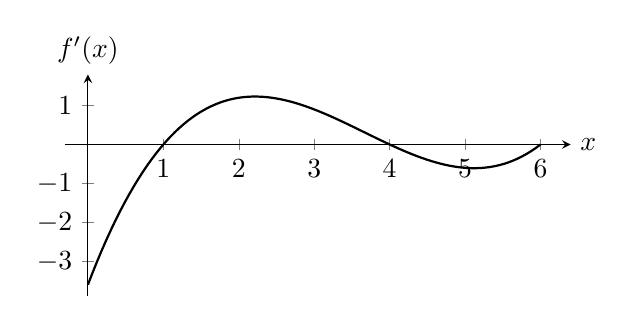
\begin{tikzpicture}
\begin{axis}[width=8cm,height=4.4cm,axis lines=middle,xmin=-0.3,xmax=6.4,ymin=-3.9,ymax=1.8,xtick={1,...,6},ytick={-3,-2,-1,1},xlabel={$x$},ylabel={$f'(x)$},
 every axis x label/.style={at={(ticklabel* cs:1)},anchor=west},every axis y label/.style={at={(ticklabel* cs:1)},anchor=south}]
\addplot[thick,domain=0:6,samples=100]{0.15*(x-1)*(x-4)*(x-6)};
\end{axis}
\end{tikzpicture}
\end{center}
The graph shows $f'$ on $[0,6]$ with zeros at 1, 4, 6. $f$ decreases on $(0,1)$, increases on $(1,4)$, decreases on $(4,6)$: relative min at $x=1$, relative max at $x=4$ ($f'$ changes $-\to+$ and $+\to-$). $f'$ turns at about $x=2.2$ and $x=5.1$: inflection points of $f$ there.
\end{example}

\section{Optimization (5.10--5.11)}

\begin{rulebox}{R5.10}{Optimization procedure}
(1) Write the quantity to optimize as a function of \emph{one} variable, using the constraint. (2) State the domain. (3) Find critical points. (4) Justify the absolute extremum: candidates test on a closed interval, or a single critical point with a sign change of the derivative (first derivative test for absolute extrema). Answer the question that was asked (the dimension, or the maximum value).
\end{rulebox}

\begin{example}{a fenced field along a river}
600 m of fence for three sides of a rectangle along a river. Area $A=x(600-2x)$, $0<x<300$. $A'=600-4x=0$ at $x=150$; $A'$ changes $+\to-$, the only critical point, so it gives the absolute max. \answer{$150\times300$ m, area 45{,}000 m$^2$.}
\end{example}

\section{Behaviors of implicit relations (5.12)}

\begin{rulebox}{R5.11}{Implicit curves}
For a curve defined implicitly, the same logic applies with $\frac{dy}{dx}$ from Unit 3: $\frac{dy}{dx}>0$ means the curve rises through that point, horizontal tangents occur where the numerator is 0, and the sign of $\frac{d^2y}{dx^2}$ at a point gives concavity there.
\end{rulebox}

\section{Common errors}
\begin{itemize}
\item MVT or IVT conclusions without stating continuity and differentiability (R5.1).
\item Calling $f''(c)=0$ an inflection point without a sign change (R5.7).
\item Reading a graph of $f'$ as if it were $f$: the \emph{top} of the $f'$ graph is an inflection point of $f$, not a maximum (R5.9).
\item Forgetting the endpoints in the candidates test (R5.6).
\item Justifying with ``the graph goes up'': the scoring guide wants a statement about $f'$ or $f''$ (R5.5, R5.9).
\end{itemize}

\end{document}
